\chapter{Implementação e Testes} \label{cap:development}
Neste capítulo, são apresentados os detalhes de implementação e testes do aplicativo. Primeiramente a implementação do aplicativo iOS é detalhada. Em seguida, é abordada a integração de todos os sistemas de software que compõe a aplicação. Por último, as implementações de testes automatizados de interface gráfica são apresentadas. 

\section{Banco de Dados}
O banco de dados da aplicação está localizado na nuvem, através do serviço de acesso remoto da Amazon. O banco de dados projetado segue o modelo relacional, o qual foi julgado suficiente para representar os dados armazenados na aplicação e por ser extensamente utilizado em aplicações similares (que requerem cadastro e armazenamento de dados de usuários e outras entidades).

A Figura \ref{fig:database} ilustra o modelo de dados projetado através do diagrama de entidades. O modelo de dados está centrado nas entidades de usuário ("User"), academia ("Gym") e agendamento ("Booking") de forma a captar a principal funcionalidade da aplicação que é conectar treinadores (usuários) e academias através de agendamentos de treinos.

\begin{figure}[H]
    \centering
    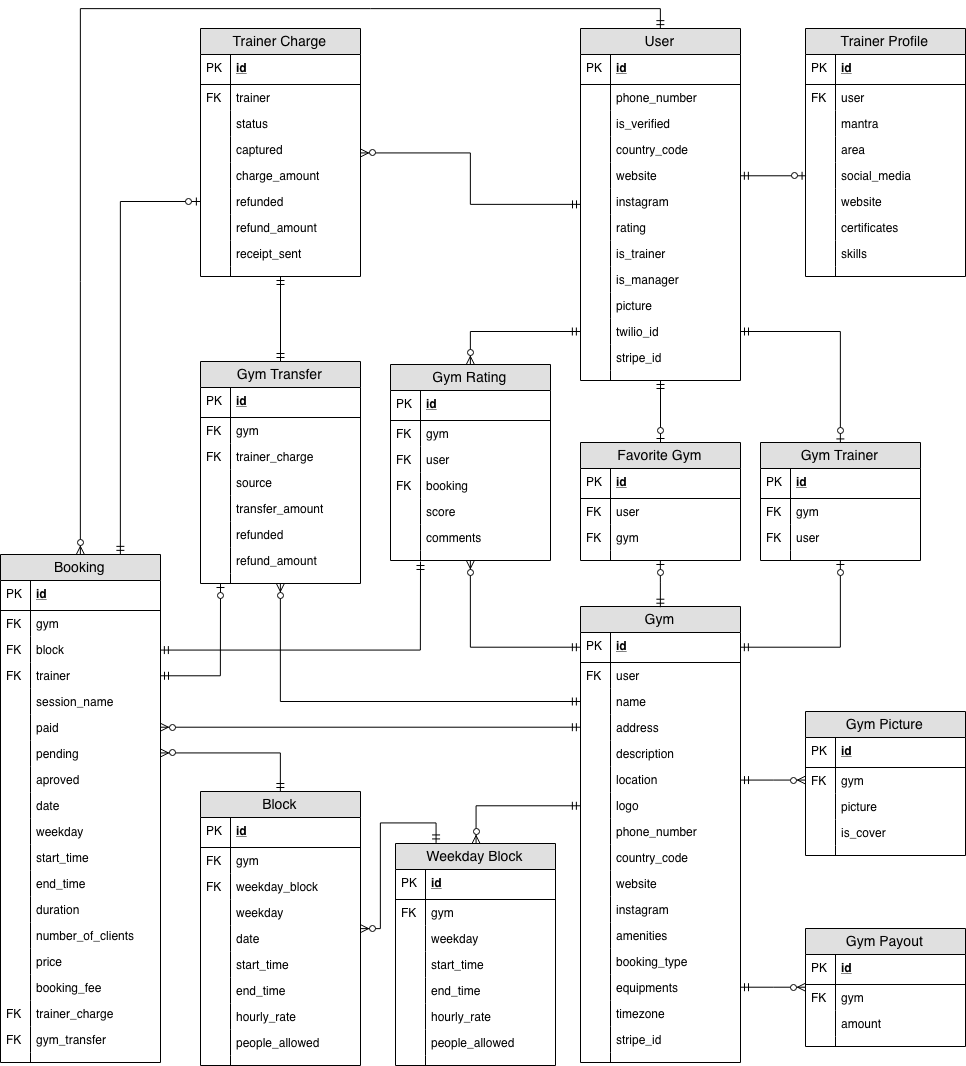
\includegraphics[width=0.8\textwidth]{pfc/figuras/database-schema.png}
    \caption{Diagrama do modelo de dados relacional}
    \label{fig:database}
\end{figure}

\section{Aplicativo iOS}
Nesta secção são apresentados os detalhes de cada camada da arquitetura do aplicativo iOS, com exemplos de implementação. Em seguida, são apresentados os critérios de avaliação das implementações. Por fim, são apresentados os desafios e dificuldades da implementação do aplicativo iOS.

% *******
% Modelos
% *******
\subsection{\textit{Model}: Representação de dados}
Os dados da aplicação são representados localmente no aplicativo iOS através de \textit{struct}'s, estrutura de dado da linguagem Swift. Uma \textit{struct} no Swift permite definir propriedades e armazenar valores, definir métodos e inicializadores, além de permitir a conformação com protocolos. Os dados apresentados no aplicativos são provenientes dos retornos das chamadas de API's e são armazenados, em sua maioria, de forma volátil no aplicativo, na memória do dispositivo. Apenas alguns dados são persistidos no dispositivo: os dados do modelo de usuário e academia são mantidos para acesso rápido; o \textit{token} de autenticação do usuário também é mantido no dispositivo para que o mesmo possa manter sua sessão atual ativa, mesmo após fechar o aplicativo.


A Figura \ref{fig:user-model} exemplifica a representação de dados no aplicativo através do modelo de usuário. A \textit{struct} contém as propriedades relacionadas ao usuário, com os respectivos tipos de dados associados. O protocolo \textit{Codable} é utilizado para permitir a tradução automática de dados da API, convertendo-os em uma instância da \textit{struct}. O modelo de usuário contém ainda uma variável computada ("fullName"), ou seja, calculada a partir de propriedades armazenadas.

\begin{figure}[H]
    \centering
    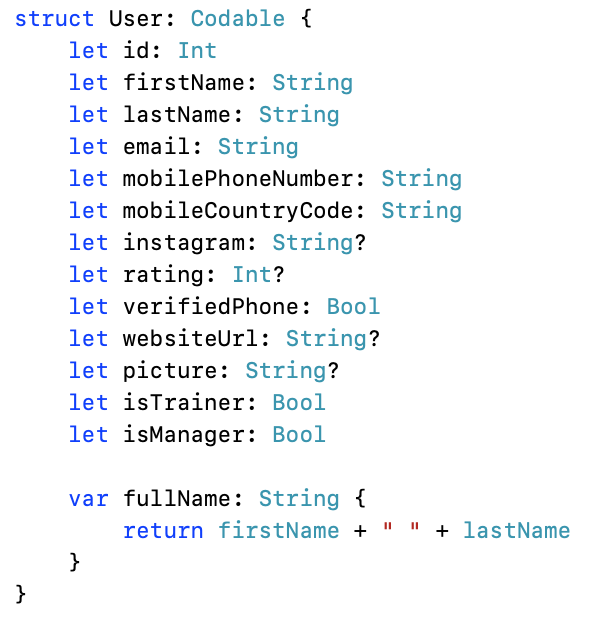
\includegraphics[width=0.8\textwidth]{pfc/figuras/user-model.png}
    \caption{Exemplo de modelo local de dados no aplicativo iOS}
    \label{fig:user-model}
\end{figure}

% **********
% Controller
% **********
\subsection{\textit{Controller}: Lógica e Tratamento de Ações}
A camada que controla a parte lógica do aplicativo e o tratamento de ações (em resposta à interações com o usuário) foi implementada com \textit{UIViewControllers}, classe base para controladores fornecida pelo framework UIKit. Os controladores foram separados em classes que tratam, em linhas gerais, da lógica de uma tela específica do aplicativo. Assim, os mesmos são responsáveis por definir o comportamento das telas em cada etapa de seu ciclo de vida, além de responder às interações associadas a elementos da interface em questão. Também realizam a chamada de métodos da camada de redes do aplicativo, em que chamadas de API's são feitas, e atualizam a interface gráfica com os dados recebidos.

A Figura \ref{fig:controller-example} contém um trecho de código de um exemplo de controlador. O exemplo implementa o controlador responsável pela lógica do dashboard de treinadores. No trecho de código é possível visualizar a propriedade "dashboard", que quando sobrescrita, chama um método para atualizar os dados da interface gráfica ("setupDashboardData()"). Também é possível ver o controle do comportamento da tela nas etapas de ciclo de vida em que: teve seus elementos de interface carregados ("viewDidLoad()") e está prestes a ser renderizada ("viewWillAppear()"). Nestas etapas, são chamados diversos métodos que controlam o comportamento da tela, como configuração de aspectos de aparência ("setupView()"), atualização de textos de acordo com a localização do dispositivo ("setupLocalizables()"), entre outros.

\begin{figure}[H]
    \centering
    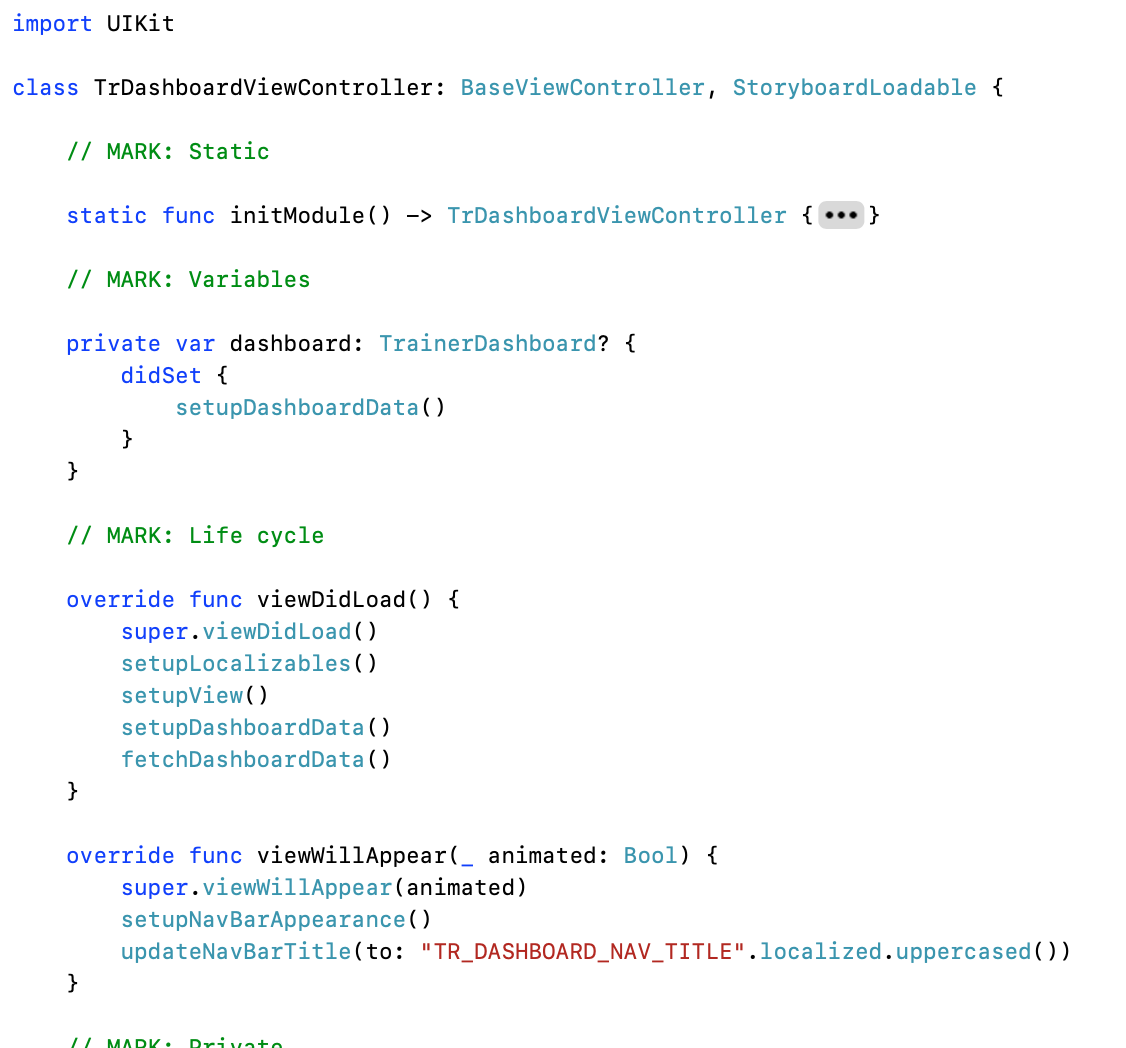
\includegraphics[width=0.8\textwidth]{pfc/figuras/ex-tr-dashboard.png}
    \caption{Exemplo de implementação de controladores no aplicativo iOS}
    \label{fig:controller-example}
\end{figure}

% *****************
% Interface Gráfica
% *****************
\subsection{\textit{View}: Interface Gráfica}
A implementação das interfaces gráficas do aplicativo foi feita principalmente com o uso de \textit{Storyboard}'s, ferramenta gráfica de construção de interfaces do Xcode. A Figura \ref{fig:storyboard} ilustra o uso de um \textit{Storyboard} para a construção da tela de entrada do aplicativo. Na parte esquerda da figura, é apresentada a hierarquia dos componentes da interface. Na região central, os elementos são dispostos na tela de acordo com o dispositivo selecionado. Na direita, encontram-se especificações de restrições de layout impostas ao componente da interface selecionado.

\begin{figure}[H]
    \centering
    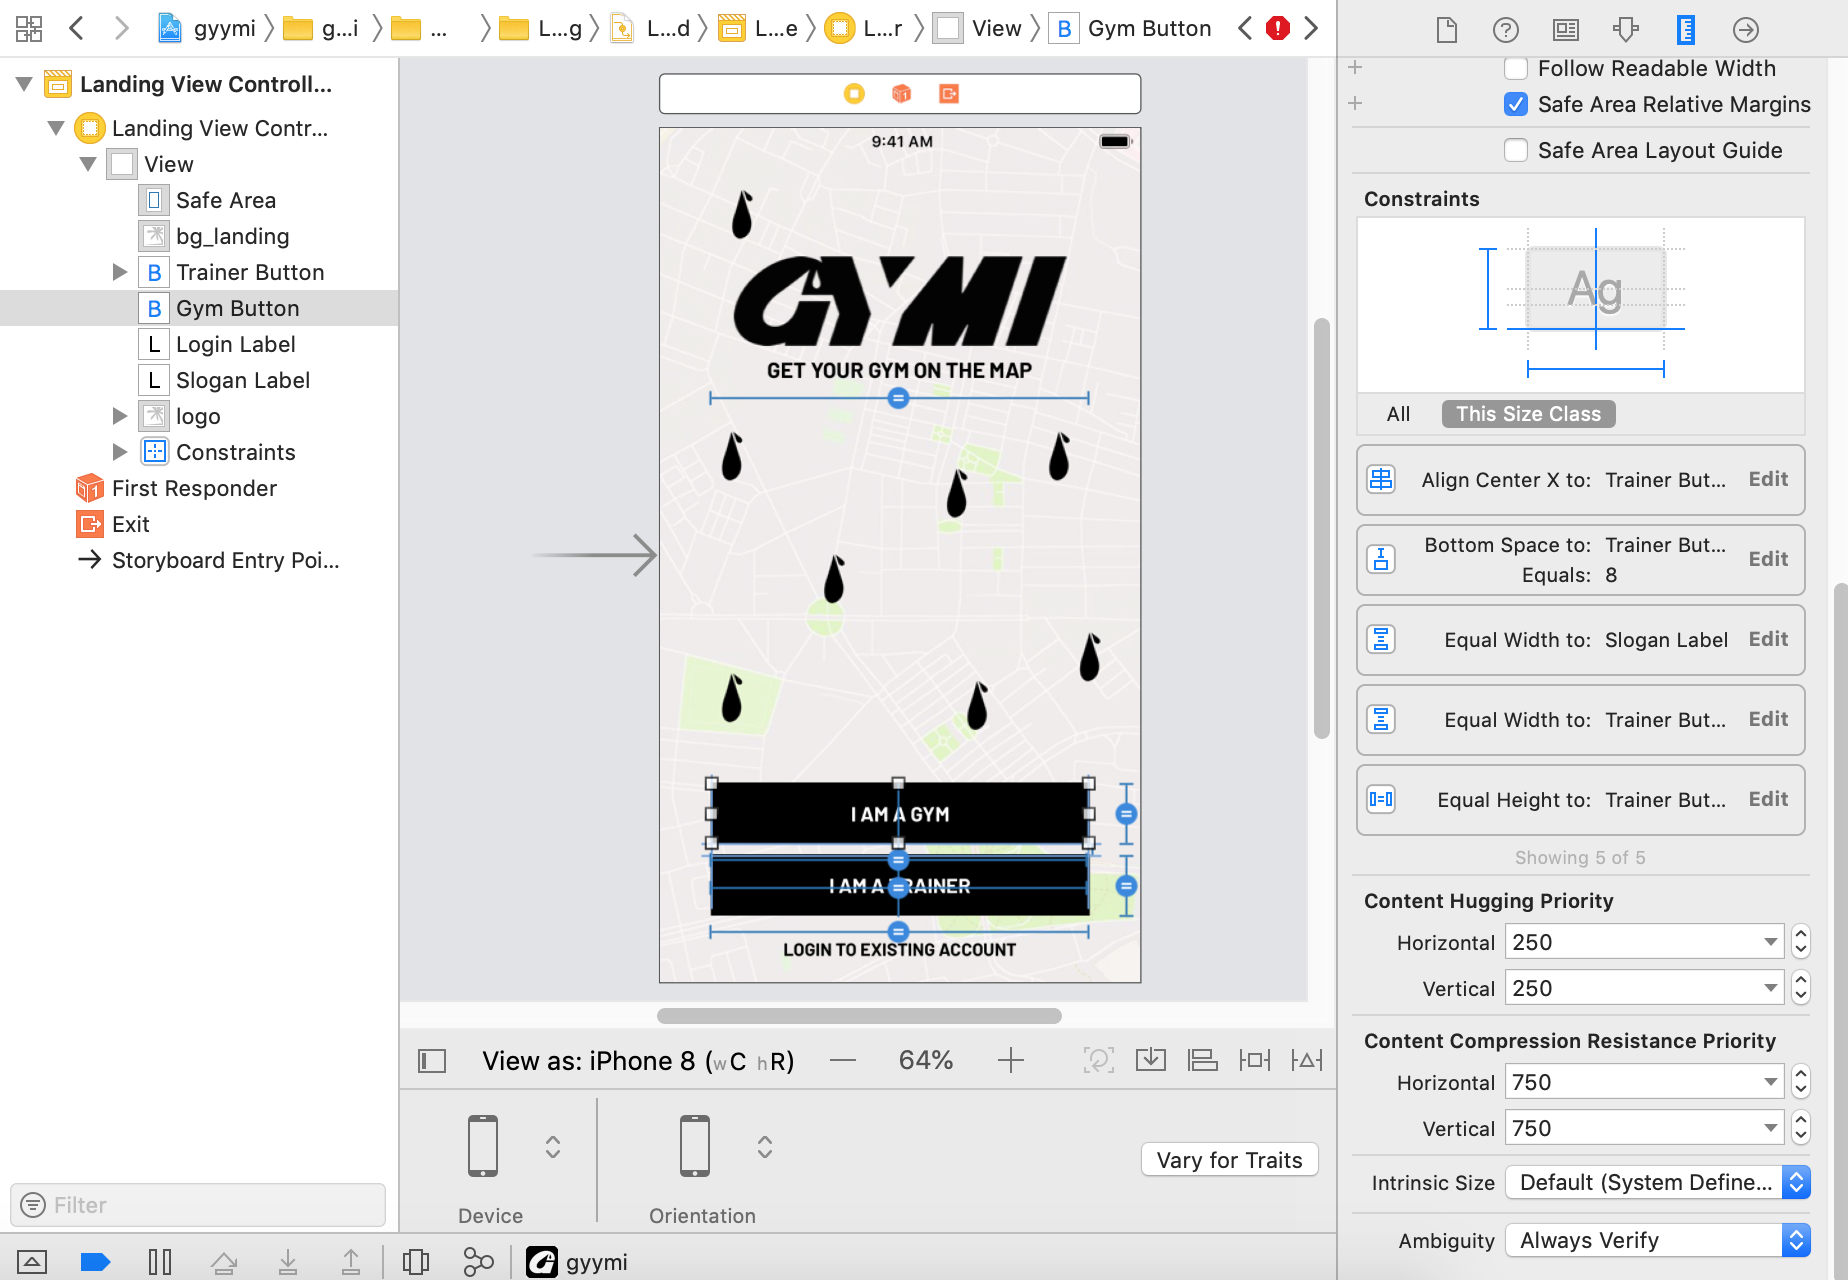
\includegraphics[width=0.8\textwidth]{pfc/figuras/storyboard.png}
    \caption{Uso de \textit{Storyboard}'s para implementação de interface gráfica}
    \label{fig:storyboard}
\end{figure}

\subsection{Critérios de Avaliação}
A implementação do aplicativo foi avaliada seguindo critérios técnicos para garantir a qualidade do produto e a conformidade com os requisitos do projeto. Alguns destes critérios e práticas adotadas para atendê-los são discutidos a seguir.

Em relação ao código, algumas abordagens foram estabelecidas para mantê-lo limpo, em conjunto com as boas práticas de programação. Foi utilizado a ferramenta \textit{SwiftLint} \todo{referenciar swiftlint} para assegurar a padronização de estilo e a conformidade com convenções estabelecidas para a escrita na linguagem Swift. Sempre que o código é compilado, avisos são gerados na IDE caso algum desvio de padrão seja encontrado no código. Boas práticas de programação também foram utilizadas para avaliar a qualidade do código, como a divisão de responsabilidades e reuso de componentes.

A avaliação da interface gráfica foi feita com base em testes de múltiplos dispositivos. Através da SDK iOS integrada ao Xcode, foi possível realizar a simulação do aplicativo em diferentes dispositivos. O critério utilizado para a aprovação de uma interface gráfica foi a avaliação positiva (conformidade com o projeto de design da aplicação e ausência de comportamentos gráficos estranhos) em pelo menos dois tipos de dispositivos de diferentes tamanhos de telas. A Figura \ref{fig:devices} ilustra o teste feito para a tela de dashboard das academias nos simuladores do iPhone SE, iPhone 7 e iPhone X.

\begin{figure}[H]
	\centering
    \begin{subfigure}[b]{0.3\textwidth}
        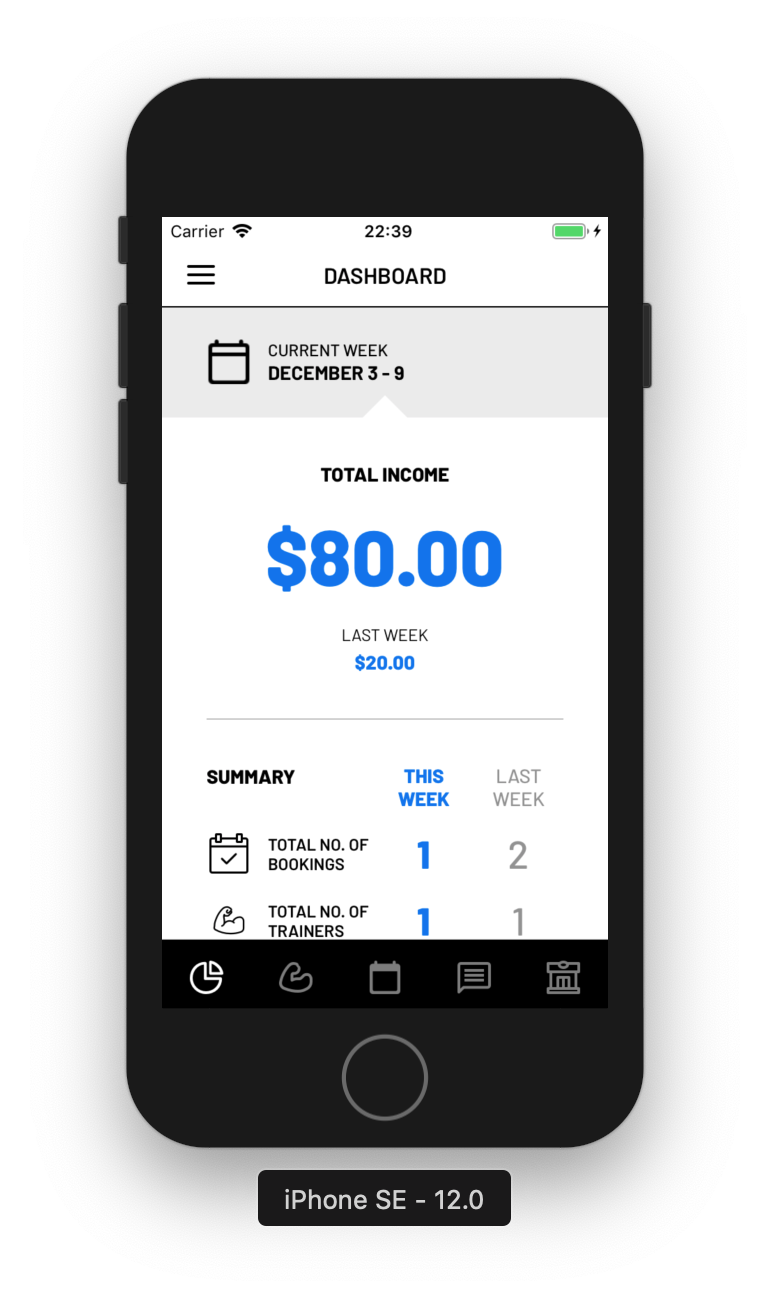
\includegraphics[width=\textwidth]{pfc/figuras/se.png}
        \caption{Simulador iPhone SE}
        \label{fig:se}
    \end{subfigure}
    ~
	\begin{subfigure}[b]{0.3\textwidth}
        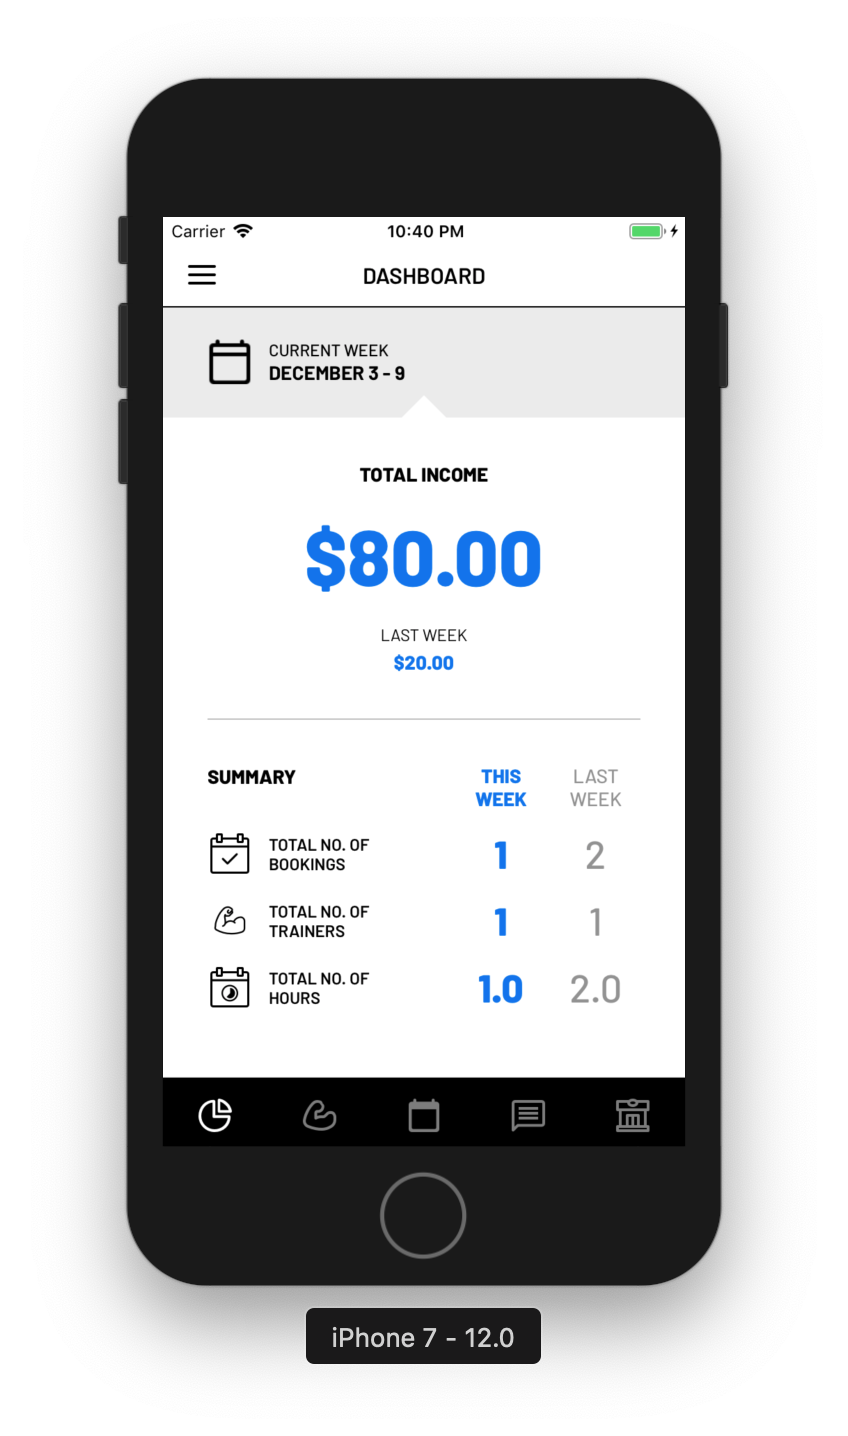
\includegraphics[width=\textwidth]{pfc/figuras/7.png}
        \caption{Simulador iPhone 7}
        \label{fig:7}
    \end{subfigure}
    ~
    \begin{subfigure}[b]{0.3\textwidth}
        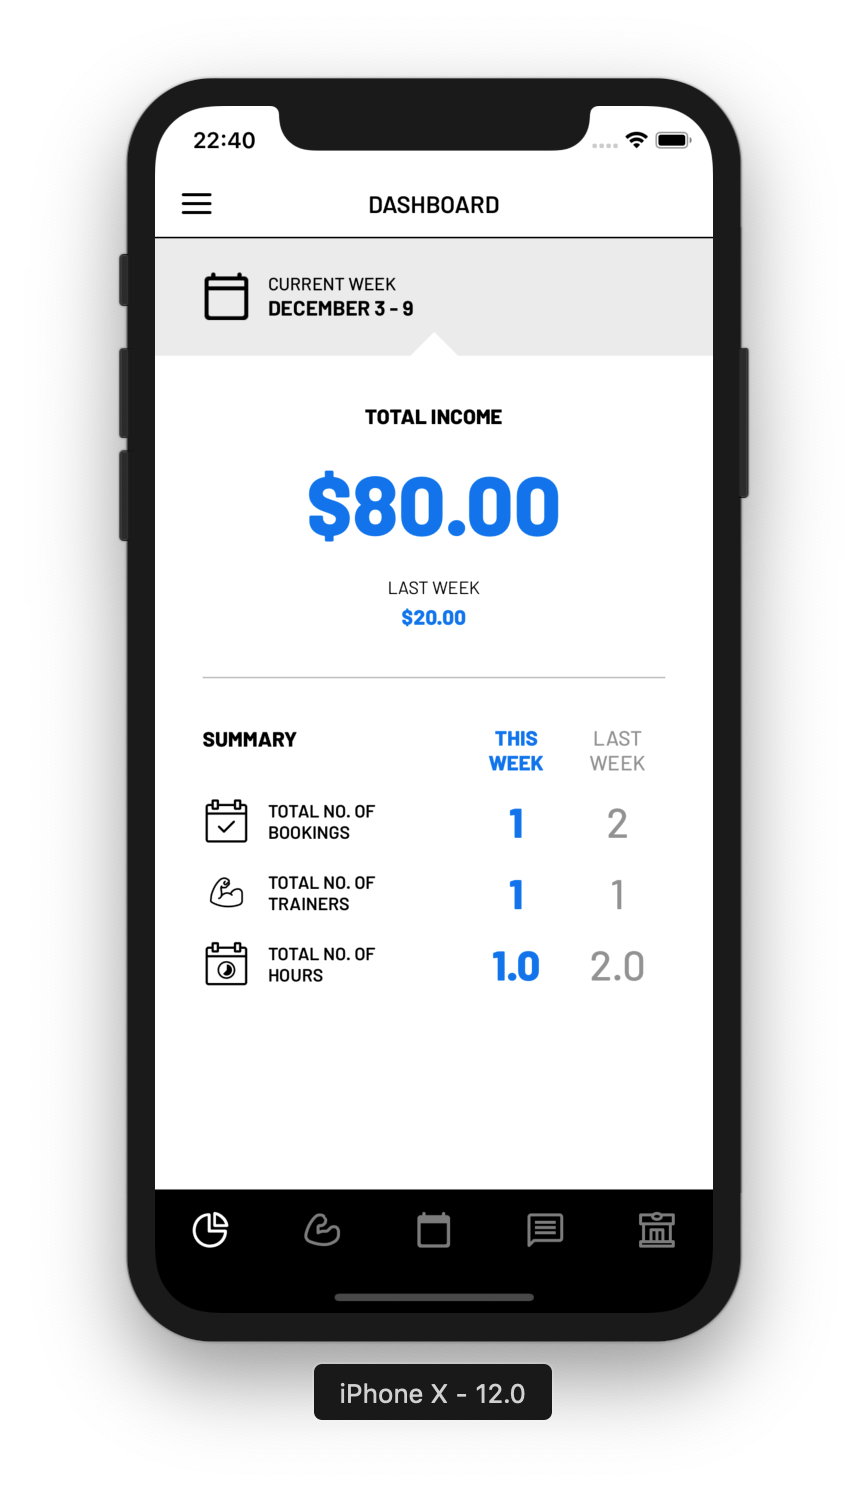
\includegraphics[width=\textwidth]{pfc/figuras/x.png}
        \caption{Simulador iPhone X}
        \label{fig:x}
    \end{subfigure}
    ~
    \caption{Uso de diferentes tipos de dispositivos}
    \label{fig:devices}
\end{figure}

\subsection{Desafios e Dificuldades de Implementação}
O desenvolvimento do aplicativo iOS apresentou alguns desafios de implementação, tanto lógicos como de interface gráfica. Alguns exemplos são apresentados a seguir.

Um dos desafios de implementação da interface gráfica do aplicativo foram as tabelas de horários e calendários (Figuras \ref{fig:gym-block}, \ref{fig:gym-booking-calendar}). A solução encontrada foi a utilização das bibliotecas \textit{SpreadsheetView} e \textit{FSCalendar} \todo{citar essas bibliotecas}, que forneceram componentes customizáveis para auxiliar o desenvolvimento.

Uma dificuldade recorrente em muitas das telas do aplicativo foi a adaptação dos elementos gráficos a diferentes tamanhos de dispositivos, principalmente aos menores aparelhos, como o iPhone SE. Essa dificuldade surgiu devido ao fato do design do projeto ter sido baseado em dispositivos maiores. Uma das soluções para alguns casos foi diferenciar o comportamento da tela baseado no tamanho do dispositivo, classificado como pequeno ou grande através de um método de auxílio.

Em relação à parte lógica do aplicativo, o tratamento de erros apresentou alguns desafios de implementação. Muitos casos de erros e validação de campos tiveram que ser tratados no momento do cadastro dos usuários (Figura \ref{fig:register-errors}). Um exemplo de solução implementada para a validação de campos foi a utilização de expressões regulares. Erros advindos de falhas nas chamadas de API's também demandaram tempo de projeto, como a falha de autenticação de usuário ilustrada na Figura \ref{fig:session-expired}, que ocorre quando o \textit{token} do usuário é inválido. Neste último caso, a solução implementada foi apresentar um aviso explicando o problema e, em seguida, forçar o logout no aplicativo.

\begin{figure}[H]
	\centering
    \begin{subfigure}[b]{0.4\textwidth}
        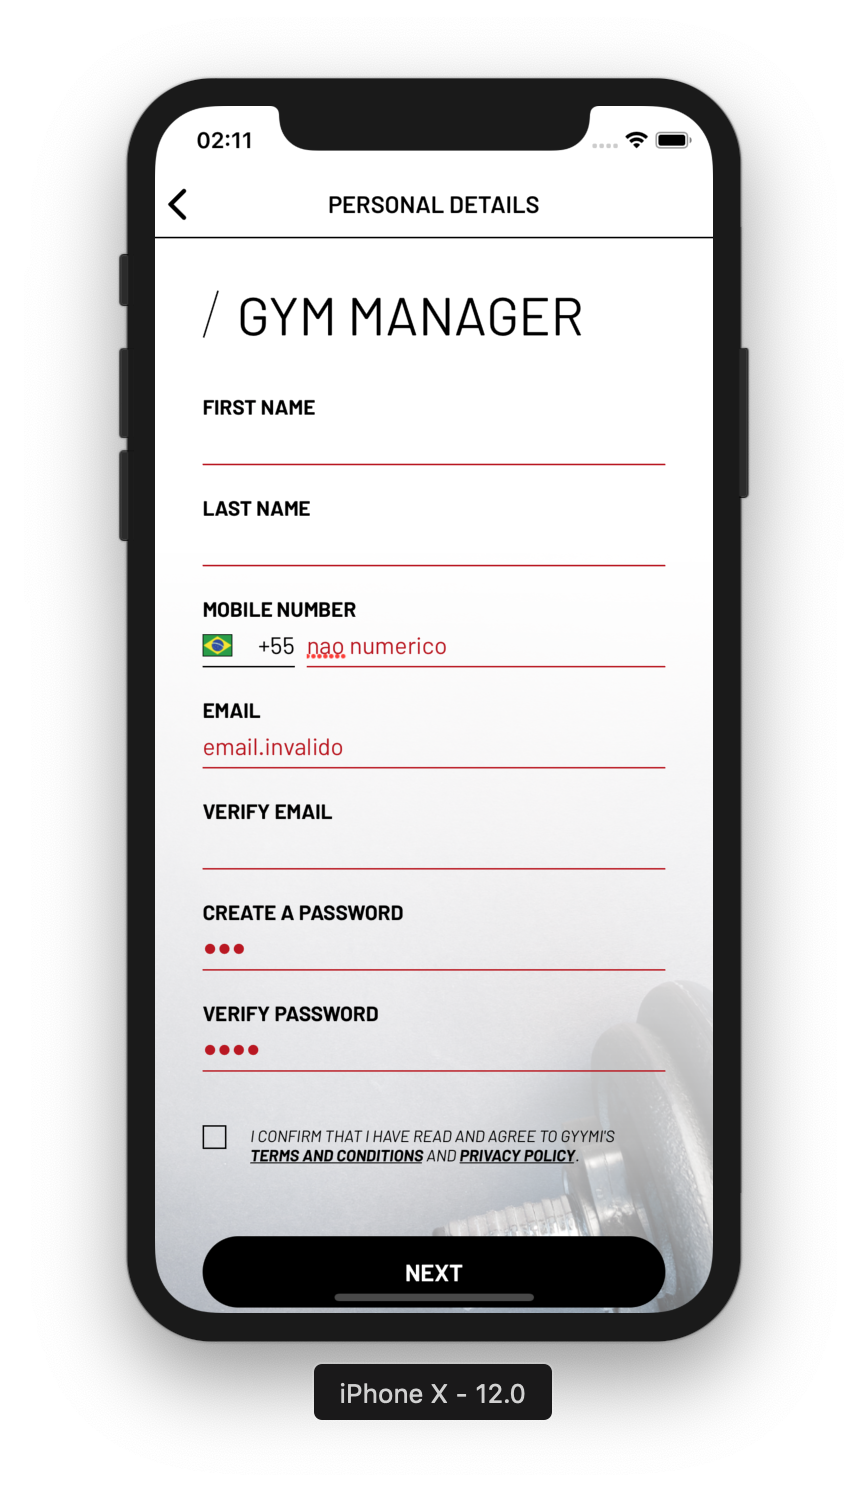
\includegraphics[width=\textwidth]{pfc/figuras/register-errors.png}
        \caption{Erros no cadastro}
        \label{fig:register-errors}
    \end{subfigure}
    ~
	\begin{subfigure}[b]{0.4\textwidth}
        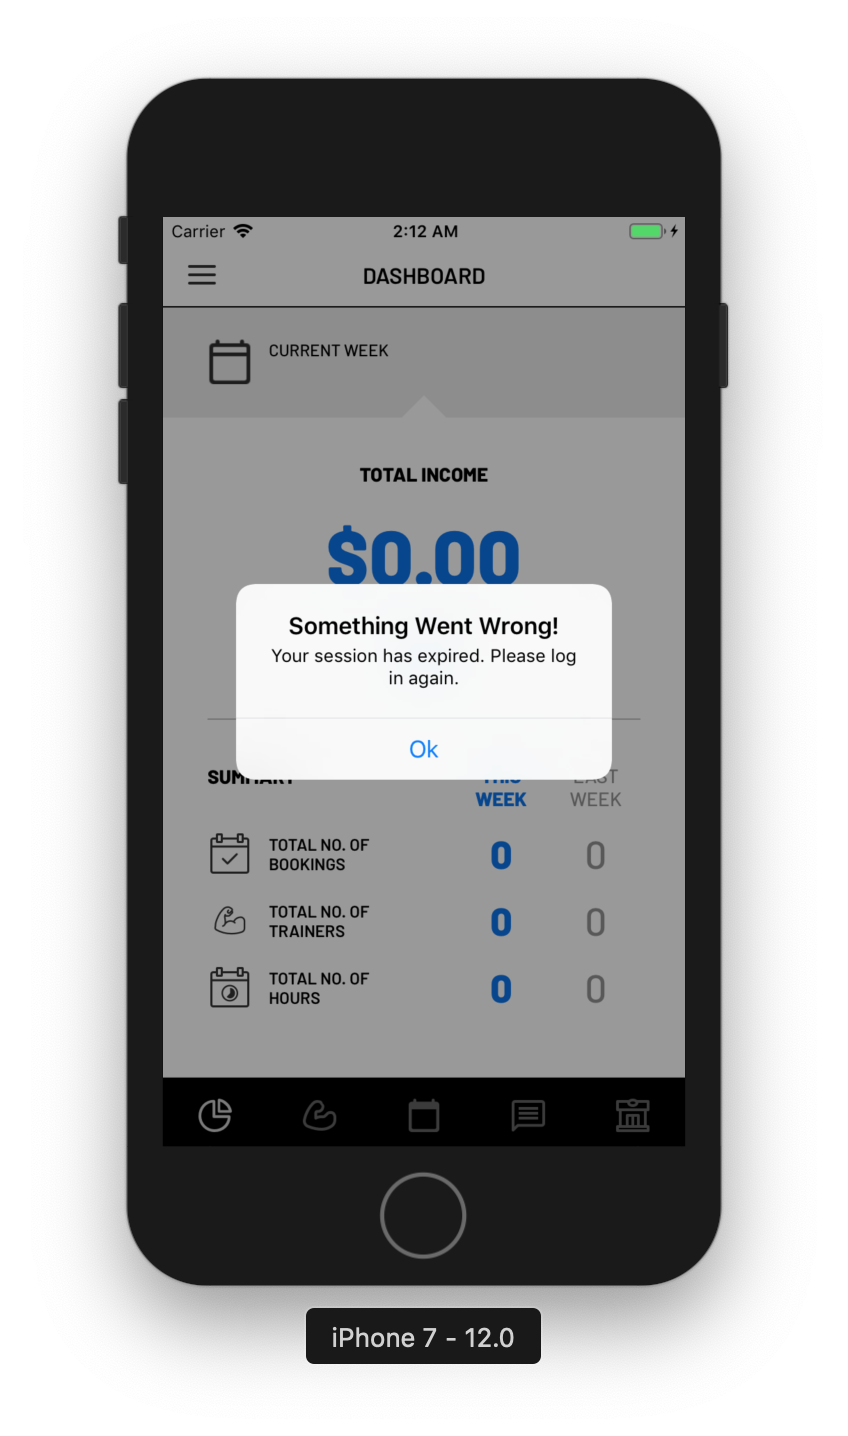
\includegraphics[width=\textwidth]{pfc/figuras/session-expired.png}
        \caption{Erro de autenticação}
        \label{fig:session-expired}
    \end{subfigure}
    ~
    \caption{Exemplos de estados de erro no aplicativo}
    \label{fig:error-states}
\end{figure}

% **********************
% Integração de Sistemas
% **********************
\section{Integração de Sistemas}
O desenvolvimento da aplicação evolveu a integração de múltiplos sistemas de software, tanto internos quanto externos. Nesta secção, primeiro é apresentada a integração com o sistema de back-end, desenvolvido internamente. Em seguida, o mesmo é feito para os sistemas externos. Por último, a ferramenta utilizada para testes das integrações feitas por RESTful API's são apresentadas. 

\subsection{Back-end}
A integração com o back-end foi feita por meio de uma API REST. A API fornece endpoints que retornam informações relacionadas à lógica de negócio da aplicação e permitem o cadastro de dados do usuário.

O formato utilizado para troca de dados foi o JSON \todo{referenciar fig json}. Este formato foi utilizado por apresentar uma notação simples para entendimento e pelo fato de ser utilizado em larga escala em integrações de serviço web. Do ponto de vista humano, a notação é de fácil visualização por não apresentar uma sintaxe verbosa. Além disso, o formato tem suporte nativo de diversas linguagens de programação, incluindo o Swift, utilizado para realizar a implementação.

\missingfigure{exemplo de json}

A API contém algumas características relacionadas à segurança do sistema. A API fornece diferentes níveis de acesso para as chamadas a fim de proteger dados sensíveis. Todo usuário recebe um \textit{token} no momento em que realiza o login ou é registrado no aplicativo. Este \textit{token} é utilizado para realizar a autenticação de chamadas da API, permitindo a identificação do usuário que realizou a requisição pelo aplicativo. Através da identificação, o back-end pode retornar ou negar o pedido de chamada de API de acordo com o nível de acesso do usuário. Além da autenticação e autorização de usuários no sistema, existem dois ambientes de uso da API: um para fase de desenvolvimento e testes, outro para o aplicativo em produção. Ambos os ambientes contêm o mesmo conjunto de chamadas de API disponíveis, distinguindo-se apenas no uso de diferentes bancos de dados (desenvolvimento e produção). Este recurso permite a separação do uso do aplicativo para fins de testes, realizados pelo time de desenvolvimento e pelo cliente, e para fins de uso real, feito pelo usuário final. A separação dos ambientes é feita a partir da diferenciação da URL base da API REST.

No código do aplicativo, as chamadas de API são feitas com o auxílio de uma biblioteca para a linguagem Swift. A biblioteca, denominada Alamofire \todo{ref alamofire}, é uma camada de abstração para a utilização de recursos de rede do sistema iOS.

O recebimento dos dados da API é feita a partir de uma tradução automática do formato JSON para objetos do Swift. A tradução é feita através da utilização de recursos nativos do Swift. Além disso, é utilizado um parâmetro de configuração que transforma a notação \textit{snake case} da API para a notação \textit{camel case}, utilizada no código.

\subsection{Serviços Externos}
O desenvolvimento do aplicativo teve como requisito a implementação dos sistemas de geolocalização, pagamento e envio de SMS. No projeto, optou-se pela utilização destes sistemas na forma de serviços devido ao grande esforço envolvido na implementação e manutenção dos mesmos. Existem diversas alternativas consolidadas há anos no mercado para cada um dos sistemas citados. As soluções escolhidas e as integrações realizadas são apresentadas a seguir. 

\subsubsection{Geolocalização}
O aplicativo apresentou como um de seus requisitos funcionais a presença de um sistema de mapa, assim como a utilização da localização do usuário. Foi escolhido o serviço de geolocalização do Google Maps \todo{referenciar google maps api}, pelo motivo do mesmo disponibilizar uma SDK para o sistema iOS de fácil utilização, com boa documentação e suporte em comunidades da internet. Para detectar a localização do usuário, utilizou-se o recurso de GPS nativo do sistema iOS, disponibilizado através do framework \textit{Core Location}, parte da camada de \textit{Core Services} do sistema operacional.

O serviço de geolocalização do Google Maps é utilizado em diversas partes do aplicativo. No momento do cadastro de uma academia, o serviço é utilizado para o preenchimento do campo endereço (Figura \ref{fig:address-field}), obrigatório para todos os estabelecimentos cadastrados na plataforma. Requisições são feitas para a API do Google Maps à medida que o usuário acrescenta caracteres no campo de endereço. Como retorno, opções de endereços semelhantes ao digitado são apresentadas na interface (Figura \ref{fig:search-delfino}). Uma vez que o usuário escolhe um dos endereços disponíveis na busca, o serviço de geolocalização retorna as coordenadas referentes ao endereço. Estas coordenadas são enviadas ao back-end para armazenamento no banco de dados, junto aos demais dados da academia, e posteriormente são utilizadas para demarcação dos estabelecimentos no mapa.

\begin{figure}[H]
	\centering
    \begin{subfigure}[b]{0.4\textwidth}
        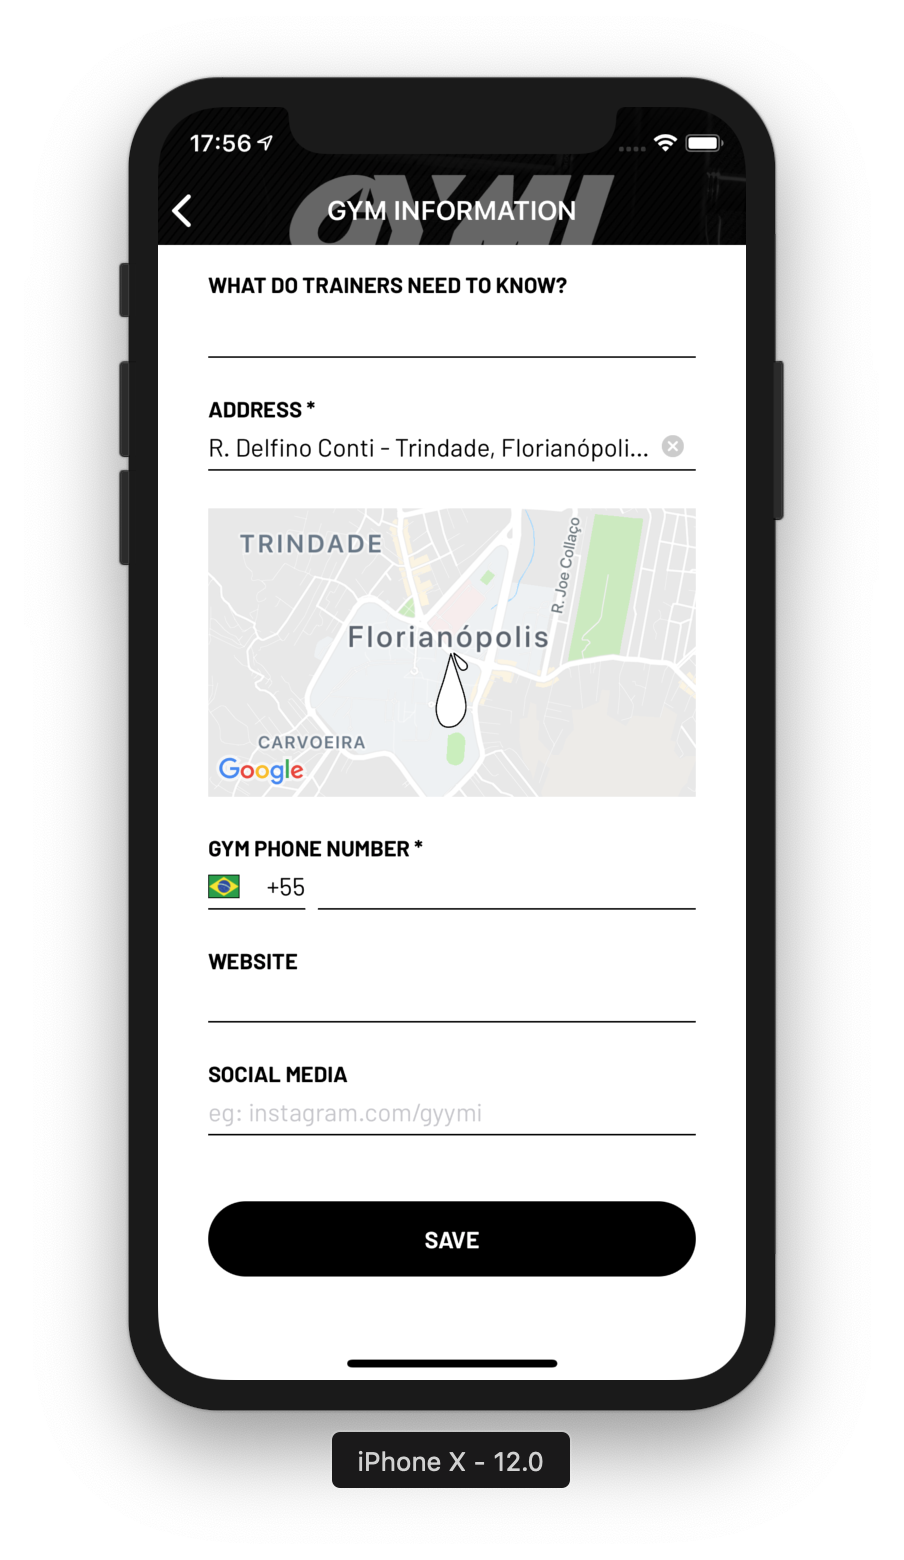
\includegraphics[width=\textwidth]{pfc/figuras/delfino-conti-2.png}
        \caption{Preenchimento do campo de endereço}
        \label{fig:address-field}
    \end{subfigure}
    ~
	\begin{subfigure}[b]{0.4\textwidth}
        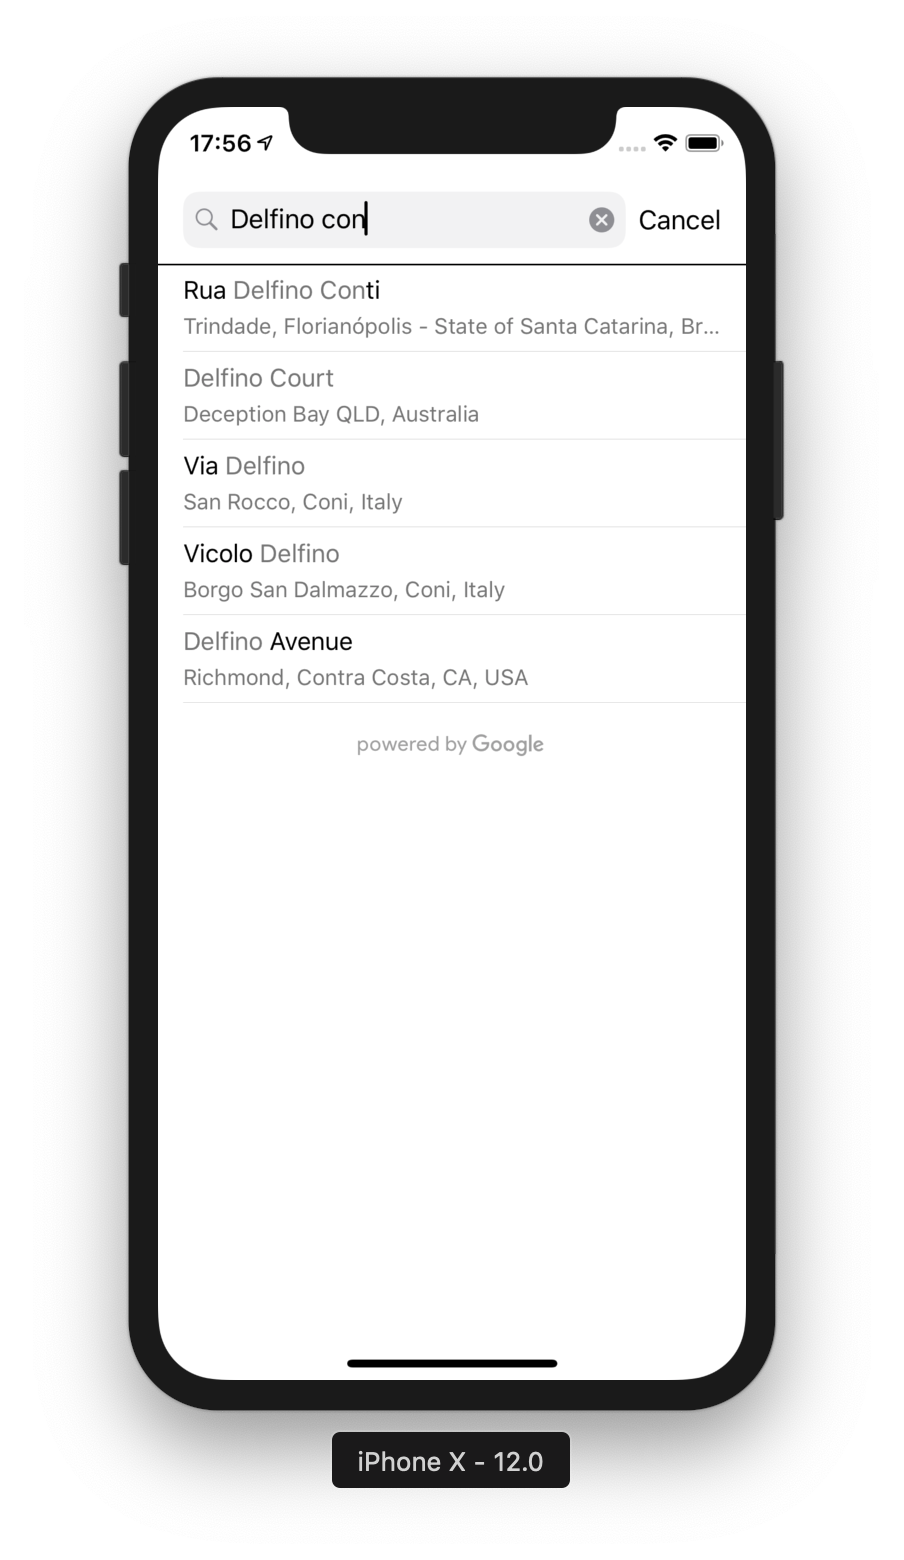
\includegraphics[width=\textwidth]{pfc/figuras/delfino-conti.png}
        \caption{Busca por endereços através da API do Google Maps}
        \label{fig:search-delfino}
    \end{subfigure}
    ~
    \caption{Etapa de preenchimento do campo endereço no cadastro de uma academia}
    \label{fig:addreess-field-fill}
\end{figure}

Outra utilização do serviço de geolocalização é o sistema de mapas, recorrente em diversas telas do aplicativo. O sistema de mapas é utilizado de maneira estática (sem a interação do usuário) nas telas de boas vindas (Figura \ref{fig:gym-welcome}), de perfil (Figuras \ref{fig:gym-profile} e \ref{fig:tr-gym-profile-view}) e de cadastro (Figura \ref{fig:address-field}) das academias e, também, na tela de confirmação de agendamento de treino (Figura \ref{fig:tr-booking-confirmed}). Na interface do treinador (Figura \ref{fig:tr-gym-search}), o mapa é renderizado na tela dinamicamente conforme a interação do usuário. O sistema de mapas permite a utilização de movimentos de pinça para alterar o zoom, além da movimentação simples do mapa através de toques na tela. Sempre que um mapa é renderizado na tela do aplicativo, uma requisição é feita ao back-end a fim de identificar as academias que estão presentes naquela região do mapa. O ponto central da região do mapa é enviado junto com um raio de busca (foi utilizado como padrão um raio de busca de $5\,km$) para o back-end. Então, uma lista com todas as academias da região é retornada e, a partir dos dados de coordenadas salvos, marcações são feitas no mapa.
                               
O framework \textit{Core Location} é utilizado em conjunto com o sistema de mapas para detectar a posição atual do usuário. Para utilizar o recurso nativo do sistema iOS, uma requisição de permissão de uso do sistema de localização do dispositivo deve ser feita ao usuário (Figura \ref{fig:gps-permission}). Em seguida, uma marcação especial é feita no mapa (ícone de músculos do braço - Figura \ref{fig:muscle-marker}) para indicar a localização corrente. A partir deste instante, um observador é configurado para que o sistema operacional emita um aviso ao aplicativo quando o usuário se movimentar. A configuração é feita com um parâmetro de precisão de $10/,m$. Assim, quando o usuário se desloca mais que esta distância, um aviso é emitido ao aplicativo e, em seguida, a posição do marcador no mapa é atualizada.

\begin{figure}[H]
	\centering
    \begin{subfigure}[b]{0.38\textwidth}
        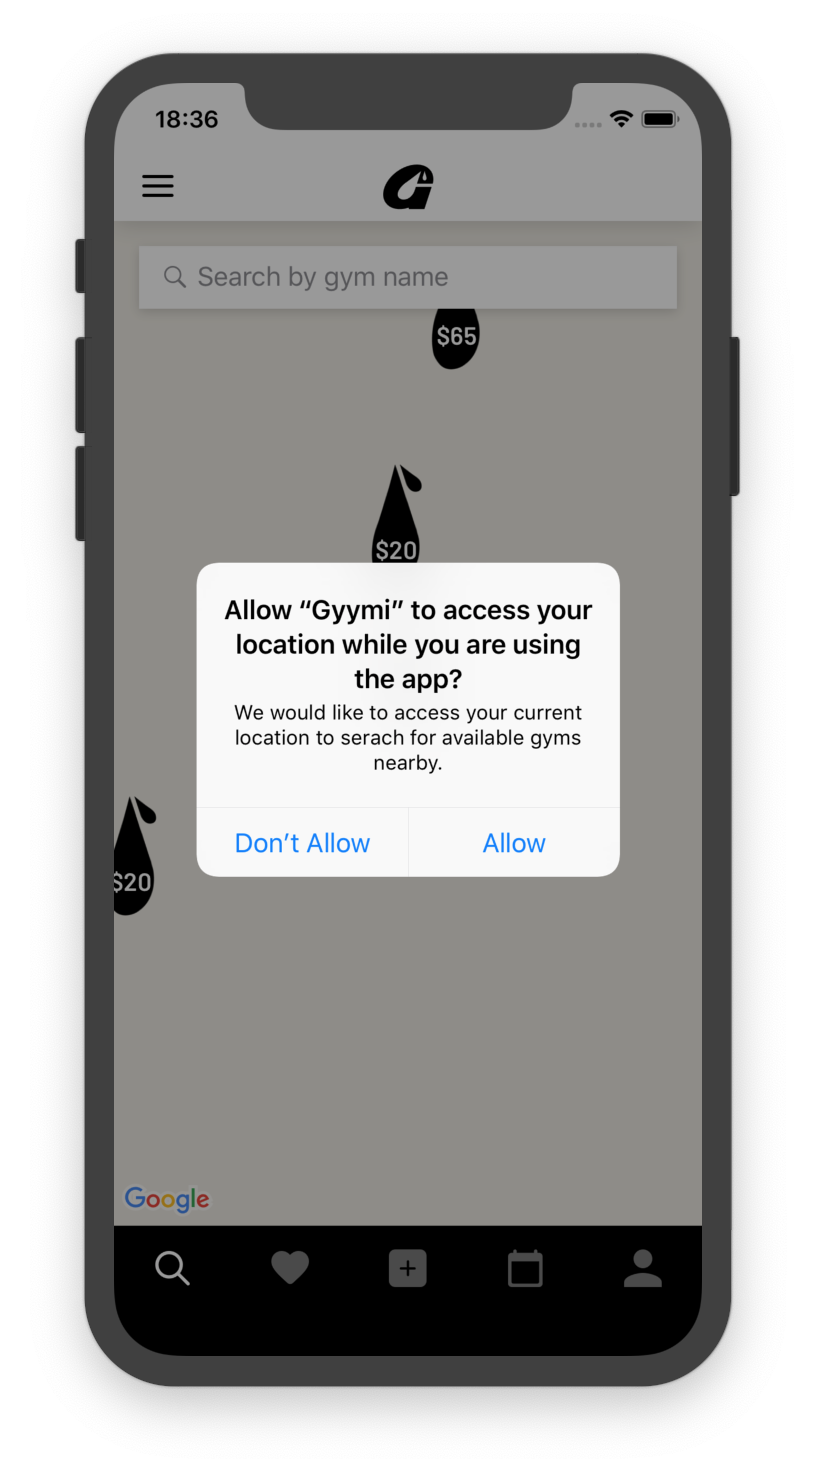
\includegraphics[width=\textwidth]{pfc/figuras/gps-permission.png}
        \caption{Permissão de uso do GPS}
        \label{fig:gps-permission}
    \end{subfigure}
    ~
	\begin{subfigure}[b]{0.4\textwidth}
        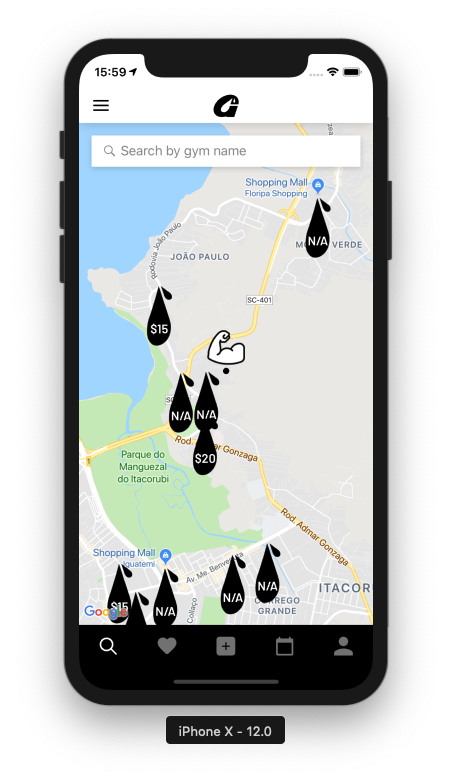
\includegraphics[width=\textwidth]{pfc/figuras/tr-home.png}
        \caption{Marcador de posição}
        \label{fig:muscle-marker}
    \end{subfigure}
    ~
    \caption{Marcação da posição atual do usuário no mapa}
    \label{fig:user-position}
\end{figure}

\subsubsection{Pagamento}
Um sistema de pagamentos foi utilizado para que as transações financeiras possam ocorrer dentro da plataforma. O serviço escolhido para implementação desta funcionalidade foi o Stripe \todo{referenciar stripe}. O serviço foi escolhido por apresentar a melhor usabilidade do ponto de vista de desenvolvimento, apresentando uma boa documentação e estrutura de API's e disponibilização de SDK para iOS com diversos recursos embutidos, como validação de campos de cartão de crédito.

O funcionamento do sistema de pagamentos da aplicação é ilustrado na Figura \ref{fig:payment-system}. Por questões de segurança, nenhum dado sensível (como número do cartão de crédito ou conta bancária) é armazenado no banco de dados da aplicação. Esta tarefa é delegada ao Stripe, assim como a realização de todas as transações financeiras. Na plataforma do Stripe, são criadas contas virtuais para cada academia, assim como uma conta virtual do Gyymi. Além disso, um processo de \textit{tokenização} é feito para a representação dos cartões de crédito dos treinadores. A \textit{tokenização} funciona da seguinte forma (ver Figura \ref{fig:seq-diagram-token}): o usuário informa os dados do cartão através da interface gráfica do aplicativo iOS; os dados são enviados para o Stripe, onde são armazenados; um \textit{token} de identificação única para representar o cartão de crédito é gerado e enviado ao aplicativo iOS; o \textit{token} é enviado ao back-end, que após validar o mesmo com o Stripe, armazena-o no banco de dados da aplicação; por último, o back-end retorna uma resposta ao aplicativo iOS informando que o processo de \textit{tokenização} do cartão de crédito foi concluído com sucesso. Dessa forma, a aplicação pode identificar cartões de crédito cadastrados e, em sequência, emitir pedidos de transação com o uso do \textit{token}.

Existem três tipos de transações dentro do Stripe:
\begin{itemize}
    \item Cobrança: quando um pagamento é feito pelo treinador, o Stripe emite uma cobrança no cartão de crédito cadastrado.
    \item Transferência: diz respeito as transferências entre contas virtuais do Stripe. Todos os pagamentos emitidos são enviados primeiramente à conta virtual do Gyymi, que retira uma taxa do pagamento como forma de cobrança pelo serviço de intermédio e, então, repassa o restante do valor para as contas virtuais das academias.
    \item Pagamento: ao final de um intervalo de tempo pré-definido, o dinheiro das contas virtuais é repassado para as contas bancárias reais.
\end{itemize}

\begin{figure}[H]
    \centering
    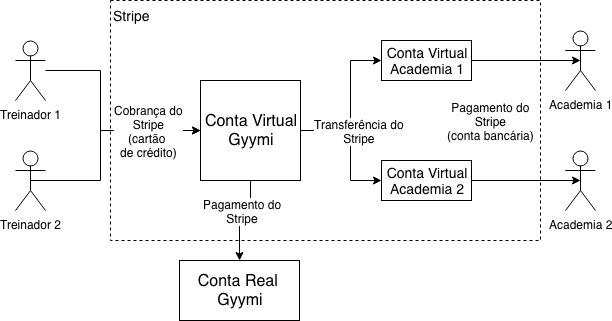
\includegraphics[width=0.8\textwidth]{pfc/figuras/payment-system-stripe.png}
    \caption{Funcionamento do sistema de pagamentos}
    \label{fig:payment-system}
\end{figure}

\begin{figure}[H]
    \centering
    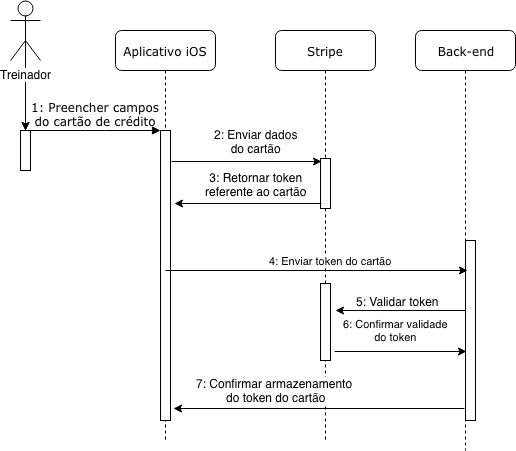
\includegraphics[width=0.8\textwidth]{pfc/figuras/seq-diagram-token.png}
    \caption{Diagrama de sequência da dinâmica de \textit{tokenização} do cartão de crédito}
    \label{fig:seq-diagram-token}
\end{figure}

A implementação dos esquemas apresentados não foi concluída para a fase piloto do aplicativo. Para o piloto, foi utilizado um ambiente fictício que o Stripe fornece para testes. Transações fictícias foram criadas no Stripe ao final dos agendamentos de treinos, emitindo-se cobranças em cartões de crédito fictícios.

\subsubsection{Envio de SMS}
O sistema de envio de SMS foi utilizado para cumprir o requisito funcional de envio de SMS para verificação de número telefônico. A verificação é feita somente no cadsatro de novos treinadores (Figura \ref{fig:register-trainer-verification}). O serviço utilizado foi o Twilio \todo{citar twilio}.

A dinâmica de envio de SMS é ilustrada no diagrama de sequência da Figura \ref{fig:seq-diagram-sms}. O sistema opera da seguinte forma: o usuário preenche o cadastro através da interface gráfica do aplicativo iOS, em especial o campo de número do celular; os dados de cadastro são enviados e validados no back-end, que faz uma chamada de API para o Twilio com um pedido de envio de SMS para o número de celular cadastrado; o usuário, então, preenche o campo de código de verificação no aplicativo com o código recebido via SMS; o código de verificação é enviado ao back-end, que realiza a validação do mesmo com o Twilio; por fim, uma confirmação da validação do código de verificação é enviada ao aplicativo iOS, permitindo que o usuário prossiga com o cadastro.

\begin{figure}[H]
    \centering
    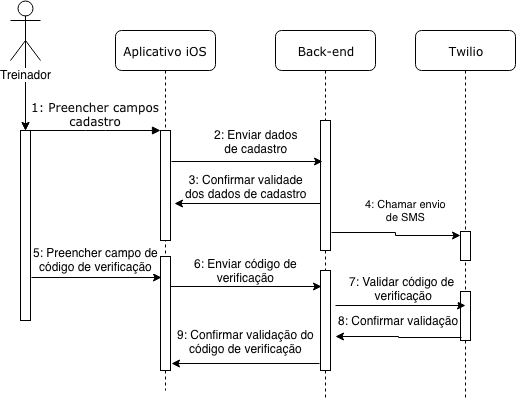
\includegraphics[width=0.8\textwidth]{pfc/figuras/seq-diagram-sms.png}
    \caption{Diagrama de sequência da dinâmica de envio de SMS para verificação de número telefônico}
    \label{fig:seq-diagram-sms}
\end{figure}

\subsection{Testes de RESTful API's}
Todas as integrações de sistemas apresentadas anteriormente foram realizadas utilizando RESTful API's. Com o intuito de agilizar e automatizar o processo de teste de chamadas de API, utilizou-se durante o projeto a ferramenta de software denominada Postman \todo{citar postman}. A ferramenta permite que conjuntos de chamadas de API's (coleções) sejam criadas, permitindo o teste das chamadas individualmente ou em conjunto (com o sequenciamento das chamadas).

A Figura \ref{fig:postman} ilustra a interface do Postman. Na esquerda, encontram-se as coleções, com as respectivas listas de chamadas de API. Na parte central superior, existem abas com as chamadas e seus parâmetros de configurações. Na parte central inferior, encontra-se um console onde a resposta da chamada é exibida.

\begin{figure}[H]
    \centering
    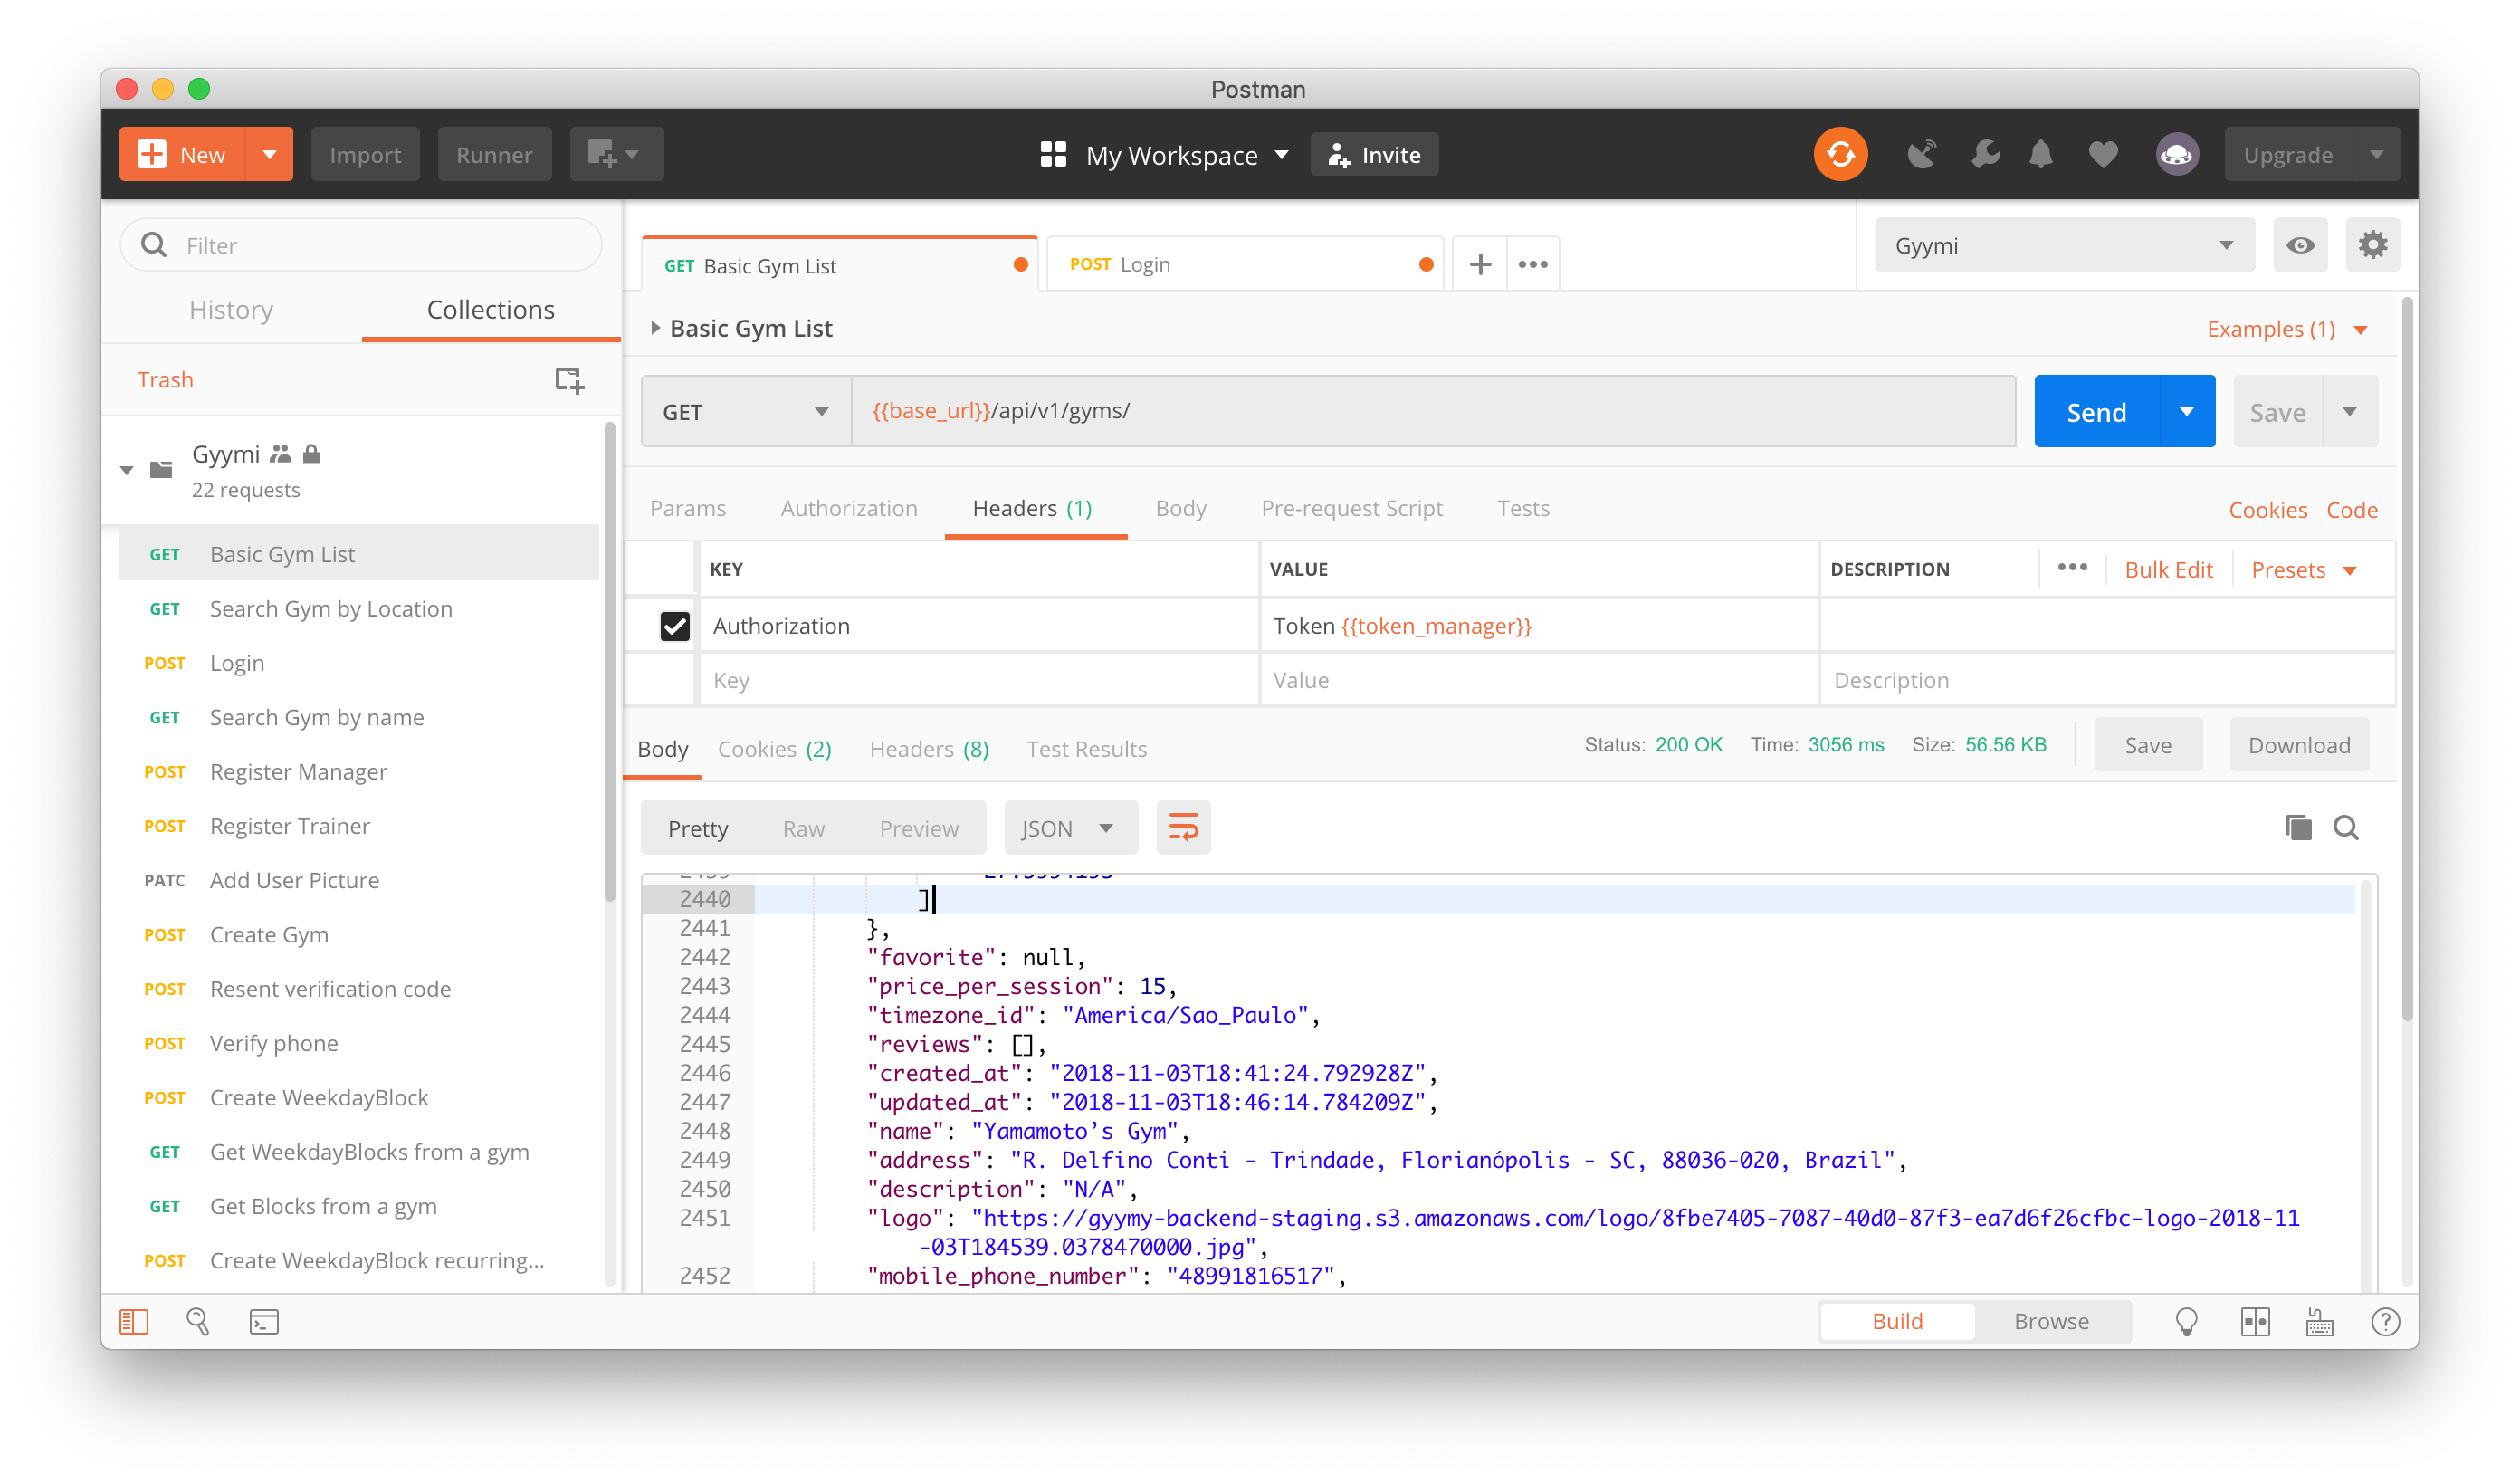
\includegraphics[width=0.8\textwidth]{pfc/figuras/postman.png}
    \caption{Postman - ferramente utilizada para testes de RESTful API's}
    \label{fig:postman}
\end{figure}

% ********************
% Testes Automatizados
% ********************
\section{Testes Automatizados de Interface Gráfica}

\subsection{Implementação dos Testes}

\subsubsection{EarlGrey}

\subsubsection{Appium}

\subsubsection{XCUITest}
